En este capítulo se presentan nuevas propuestas para resolver el problema de \texttt{\\Recuperación de Ítems Empaquetados}. El foco principal de las propuestas se centran en obtener soluciones de mejor calidad y que puedan ser generadas a partir de una mayor cantidad de elementos con respecto a lo visto en el capítulo anterior. 

Los nuevos planteos consisten en modificaciones de los algoritmos ya conocidos, trabajados en el capítulo anterior, como así también la presentación de nuevos algoritmos. Las alternativas apuntan, principalmente, a generar soluciones con paquetes más diferentes entre si, para lo cual se intenta mejorar la parte \texttt{inter} de la función objetivo.

La primera propuesta que se dará a conocer es un conjunto de mejoras aplicadas al algoritmo \texttt{Produce\allowbreak-and\allowbreak-Choose}. A su vez, en la fase de producción, más específicamente para el algoritmo jerárquico, se plantean dos mejoras: una de ellas es para reducir el orden de complejidad del algoritmo, y la otra es para equilibrar los valores \texttt{inter} e \texttt{intra} de los paquetes producidos. En cuanto a la fase de producción, la mejora que se propone es para dar más preponderancia a la parte \texttt{inter}.

Otra de las propuestas es construir la solución con una heurística que considere ambas partes de la función objetivo durante todo el proceso, y que el tiempo de ejecución sea competitivo con los otros algoritmos. Para cumplir con estos objetivos se diseñó un algoritmo goloso.

También se propone aplicar una heurísitica de búsqueda tabú, a las soluciones generadas por otros algoritmos. Con esto se intenta encontrar una mejor solución, evitando caer en máximos locales. 

\section{Produce-and-Choose}
Los algoritmos de la clase \texttt{Produce\allowbreak-and\allowbreak-Choose} generan una cierta cantidad válidos de paquetes para luego seleccionar aquellos que maximicen el valor de la función objetivo. Los cuales formarán parte de la solución.

Los parámetros del algoritmo son los del problema mencionado en~\autoref{introduccion:problemaFormal}: el conjunto de ítems $I$, el atributo complementario $\alpha$, la función de presupuesto $f: 2^{I} \rightarrow \rm I \!R$, el límite del presupuesto $\beta$, un valor $0 < \gamma < 1\ \in \rm I \!R$ para ponderar si se quiere paquetes más cohesivos o no y una cantidad $k$ de paquetes a generar. 

\begin{center}
	\begin{algorithm}[H]
	\DontPrintSemicolon
	\SetAlgoLined
		\KwData{$I,\alpha,f,\beta,k,\gamma$}
		\KwResult{Conjunto válido de $k$ paquetes}
		$cand \leftarrow ProduceBundle(I,\alpha,f,\beta)$\;
		$G \leftarrow BuildBundleGraph(cand)$\;
		\Return $ChooseBundles(k,\gamma,G)$\;
	\caption{Produce-and-Choose}\label{alg:PAC}
	\end{algorithm}
\end{center}

La función \texttt{ProduceBundle} genera un conjunto de paquetes candidatos, en las siguientes secciones se presentarán y analizarán las estrategias propuestas que se aplicaron al algoritmo jerárquico.

\texttt{BuildBundleGraph} recibe el conjunto de paquetes candidatos, transformándolo en un grafo completo con peso en las aristas y en los vértices. Cada vértice representa un paquete del conjunto de candidatos y el peso del vértice es el valor \texttt{intra}, mientras que el peso de las aristas representa el valor \texttt{inter} entre los paquetes correspondientes a cada nodo. 

Por último la función \texttt{ChooseBundles} busca el \textit{subgrafo-k} que maximice el peso de los vértices y aristas. Los vértices del \textit{subgrafo-k} corresponderán a los paquetes pertenecientes a la solución.

Como se puede observar la estructura de esta familia de algoritmos facilita la introducción de mejoras en sus dos fases críticas: generación y selección de paquetes. De este modo se podrán combinar de la mejor manera, teniendo en cuenta el objetivo de la búsqueda requerida.

\subsection{Mejoras en la generación de paquetes}
La generación de paquetes se puede realizar a través de un proceso de agrupación de un conjunto de objetos que son parecidos. Este proceso conocido como ``agrupamiento'' (\textit{clustering} en inglés) \cite{wiki:clustering} consiste en juntar objetos basándose en la información que éstos mismos describen o en sus relaciones. La finalidad es que los objetos del grupo sean similares entre sí y diferentes de los restantes grupos. Cuanto mayor sea la similitud \textbf{dentro} del conjunto (valor \texttt{intra}) y mayor sea la diferencia \textbf{entre} conjuntos el agrupamiento será mejor.

La noción de qué es un grupo correctamente constituido no puede ser definido con precisión y es por tal motivo que existe una gran cantidad de algoritmos de agrupamiento \cite{Estivill-Castro:2002:WSM:568574.568575}. Sin embargo, se puede definir como un conjunto de objetos relacionados entre sí. Teniendo en cuenta el modelo de representación usado para el problema, dependerá el tipo de algoritmo que será utilizado.

Para ejemplificar lo anteriormente mencionado, en los veinte puntos de~\autoref{res:img-howToCluster} existen más de una única forma de agruparlos que son válidas y que dependen del contexto. 

Si se quisiera agrupar por proximidad, entonces la estructura más razonable es aquella en la que se visualizarían dos grupos. A su vez cada uno de los subgrupos puede ser nuevamente particionado de acuerdo a la especificidad planteada. Por lo tanto la mejor definición de cómo se debe realizar la agrupación depende del contexto del problema.

\begin{figure}[H]
  \centering
   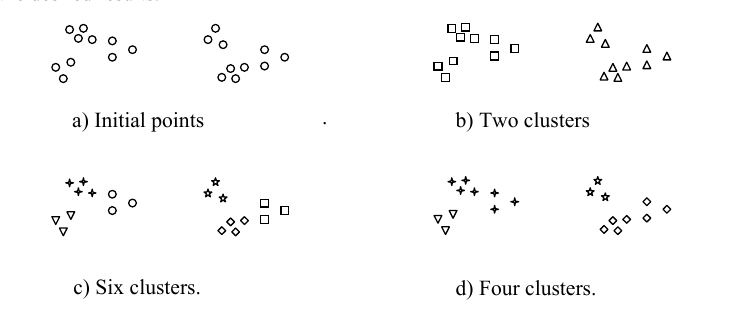
\includegraphics[width=0.8\textwidth]{img/howToCluster.png}
   \caption{}
   \label{res:img-howToCluster}
\end{figure}

De éste modo definimos el agrupamiento para que cada grupo contenga la máxima cantidad de ítems sin exceder el presupuesto. La agrupación se realiza a través de la \textbf{función de similitud} de los objetos, para que los ítems dentro del grupo sean lo más parecidos posible y así obtener paquetes cohesivos.

En la literatura se pueden encontrar diferentes tipos de algoritmos de agrupamiento, la gran mayoría puede categorizarse entre los particionales y los jerárquicos \cite{opac-b1087461}. Los métodos particionales seleccionan un número definido de $k$ centroides iniciales. Por lo tanto $k$ será el número total de grupos finales. Cada objeto será asignado al paquete que le sea más cercano y luego iterativamente los elementos serán reubicados de un grupo a otro. Este tipo de métodos requieren que la cantidad de grupos a generar sea preestablecida. 

A diferencia de los métodos particionales, los jerárquicos construyen grupos mediante la partición recursiva de los grupos de objetos y no requieren predefinir una cantidad de grupos a generar. A su vez estas técnicas se suelen subdividir en dos estrategias: aglomerativas y divisivas, las cuales serán detalladas más adelante.

En esta tesis se plantean dos mejoras para el algoritmo jerárquico \textit{Constrained hierarchical agglomerative clustering} presentado en el artículo \cite{journals/tkde/Amer-YahiaBCFMZ14}: 
\begin{enumerate}
	\item La elección en cada iteración de la estrategia para combinar \textit{clusters}.
	\item La complejidad algorítmica.
\end{enumerate}
En las próximas secciones se describirán detalladamente las mejoras propuestas.

En relación al algoritmo \textit{BOBO}, también descripto en la publicación del párrafo anterior, se mantuvo sin cambios en pos de realizar comparaciones entre los resultados obtenidos a través de las mejoras propuestas y las obtenidas mediante la implementación original.

\subsubsection{Bundles One-By-One}
El método \texttt{BOBO-k}, que está inspirado en k-means, consiste en generar $k$ paquetes del conjunto de $n$ ítems. El algoritmo comienza con todos los ítems del conjunto $I$ como posibles pivotes $P$. Se selecciona un pivote de $P$ y con los elementos de $I$ se genera un paquete válido ``alrededor'' de éste; en caso que el paquete generado sea suficientemente bueno se agrega al conjunto de candidatos, en tanto los ítems del paquete se eliminan de $I$. La generación de paquetes continúa hasta que se cumpla el criterio de parada, que es generar $k$ paquetes válidos.

\begin{center}
	\begin{algorithm}[H]
	\DontPrintSemicolon
	\SetAlgoLined
		\KwData{$I,\alpha,f,\beta,\mu,\text{ cantidad de paquetes }c$}
		\KwResult{Conjunto válido de paquetes}
		$pivots \leftarrow I$\;
		$cand \leftarrow \emptyset$\;
		\While{$ \left|C\right| < c\ and\ P \neq \emptyset$}{
			$pivot \leftarrow SelectPivot(pivots)$\;
			$bundle \leftarrow BuildBundle(pivot,I,\alpha,f,\beta)$\;
			\eIf{$Score(bundle) \geq \mu$}{
				$cand \leftarrow cand \cup \left\{bundle\right\}$\;
				$I \leftarrow I \setminus \left\{bundle\right\}$\;
				$pivots \leftarrow pivots \setminus \left\{pivot\right\}$\;
			}
			{
				$pivots \leftarrow pivots \setminus \left\{pivot\right\}$\;
			}
		}
		\Return $cand$\;
	\caption{BOBO-k}\label{alg:bobo}
	\end{algorithm}
\end{center}

La función \texttt{selectPivote} selecciona un pivote perteneciente al conjunto de pivotes, en este trabajo se siguió con la recomendación citada en \cite{Zhang:2002:ESI:638644.638646}, la cuál dice que la selección sea aleatoria. La función \texttt{BuildBundle} genera un paquete a partir del pivote. Se trata de una función que implementa un algoritmo goloso dado que en cada iteración se agrega al paquete que se genera el ítem del conjunto $I$ que maximiza la función intra y que cumple con las restricciones de la complementariedad y el presupuesto. La función \texttt{Score} calcula el valor intra del paquete. Se dice que un paquete es suficientemente bueno si el valor intra supera el umbral establecido por $\mu$.

\subsubsection{Constrained hierarchical agglomerative clustering}
Anteriormente se indicó que el agrupamiento jerárquico suele clasificarse en algoritmos \textit{aglomerativo} y \textit{divisivo}. El aglomerativo comienza con cada objeto perteneciente a un grupo unitario y en cada iteración se unen dos grupos generando un grupo nuevo. Este algoritmo es conocido como \textit{hierarchical agglomerative clustering} (HAC) \cite{journals/tkde/Amer-YahiaBCFMZ14}. 

La estrategia divisiva, en cambio, comienza con todos los objetos en un mismo grupo y en cada paso se realiza la división de uno de los grupos.

Comúnmente a los algoritmos algomerativos (HAC desde ahora en adelante) se los puede visualizar como un dendrograma, como se ve en la~\autoref{nuevaspropuestas:dendograma1}: en el eje X se encuentran los objetos que van a ser agrupados y en la coordenada Y se halla la distancia en la que los elementos se unirán. Las uniones de los objetos se representan mediante una línea vertical que comienza a la altura de la distancia en la que los grupos han sido unidos. Por ejemplo, en la figura mencionada, el grupo \textit{4} se une al \textit{5} en la distancia 2 formando el \textit{cluster B}. En un paso posterior éste último se unirá al grupo \textit{3} en una distancia cercana a 3 obteniendo el nuevo \textit{cluster C}. En cada paso se generará una nueva unión hasta que solo quede un solo grupo.

\begin{figure}[H]
  \centering
    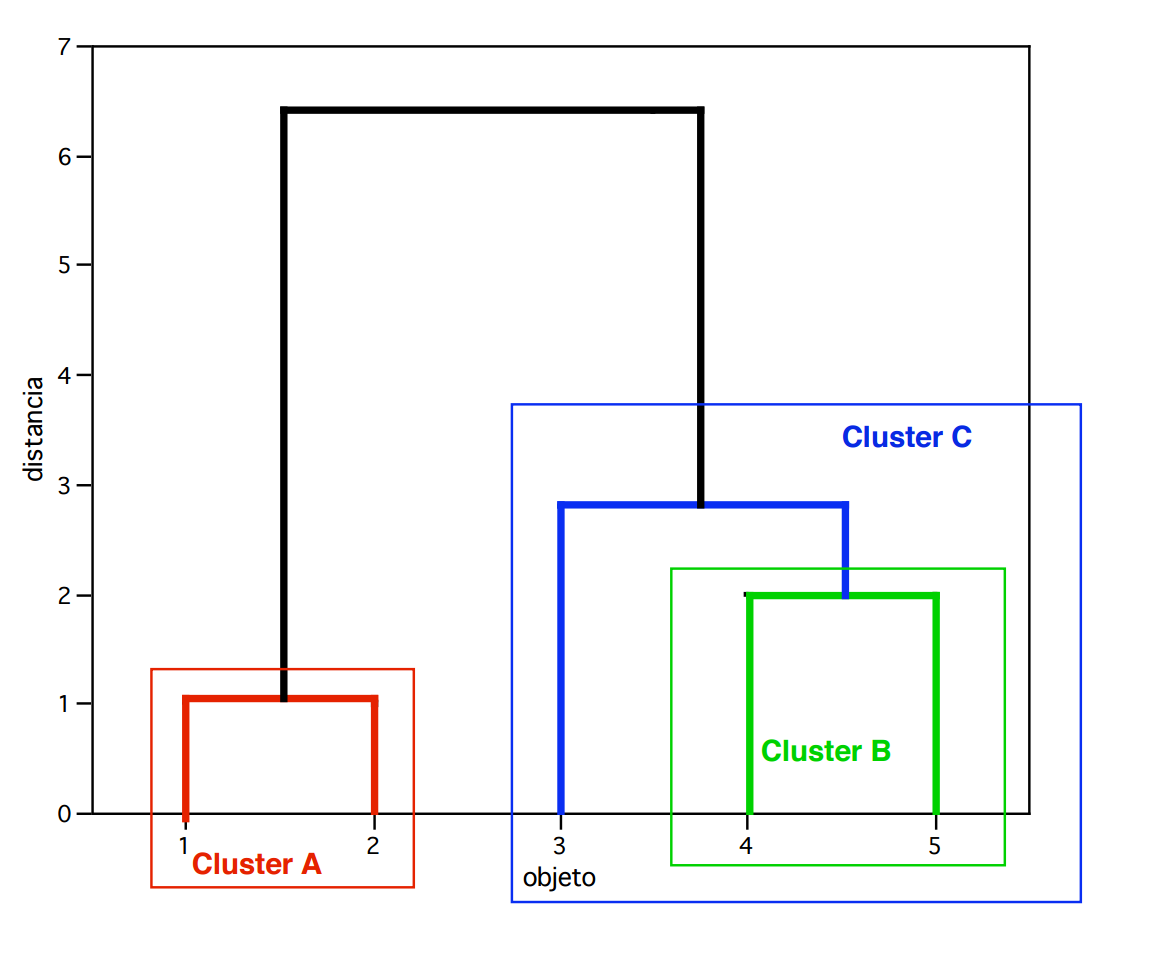
\includegraphics[width=0.5\textwidth]{img/dendograma01.png}
  \caption{Dendrograma}
  \label{nuevaspropuestas:dendograma1}
\end{figure}

Cortando el dendrograma mediante líneas horizontales se puede determinar el número de paquetes o \emph{clusters} en el que se dividirá el conjunto de objetos inicial. En la~\autoref{nuevaspropuestas:dendograma2} parte a) se puede ver que aplicando un corte en la distancia 5 se obtienen 2 paquetes, en cambio si se aplicara a una distancia mayor a 2 se obtendrían 3 paquetes como puede observarse en la parte b) de la misma figura.

\begin{figure}[H]
  \centering
    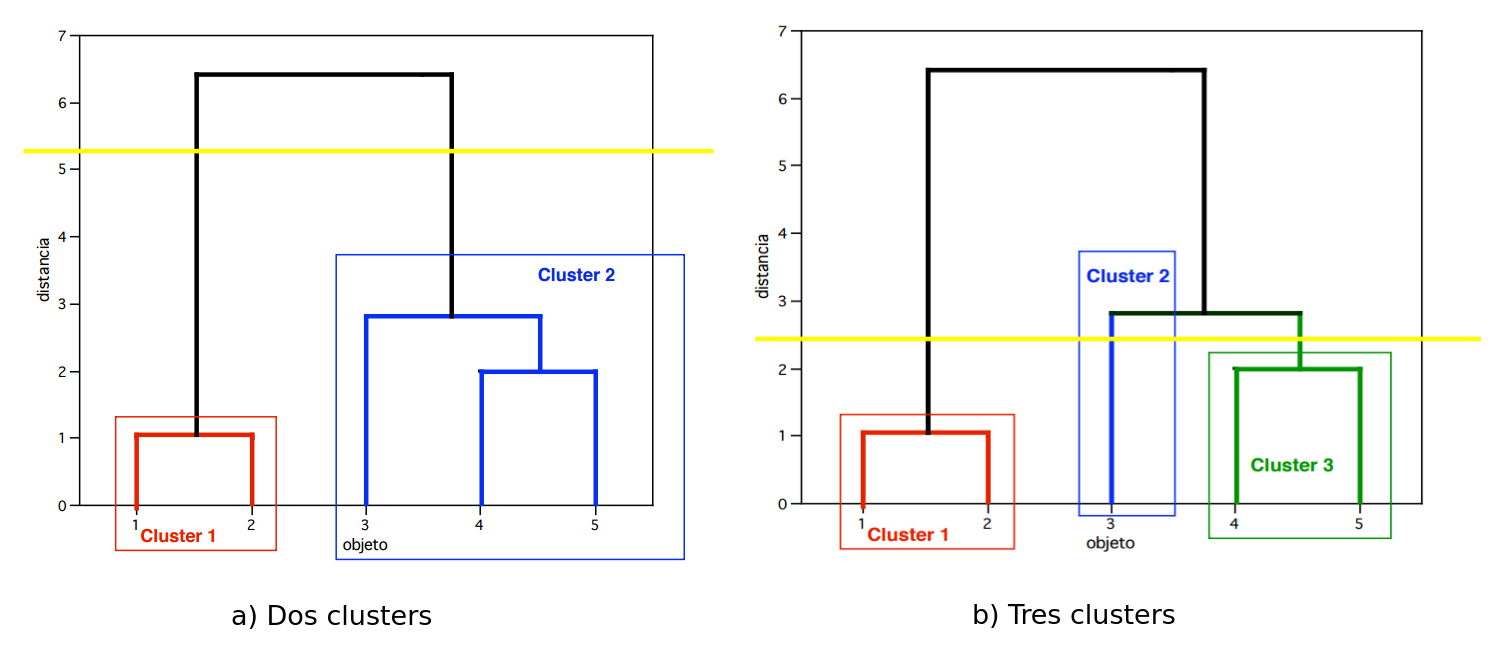
\includegraphics[width=1\textwidth]{img/dendograma02.png}
  \caption{Cortes en el dendrograma}
  \label{nuevaspropuestas:dendograma2}
\end{figure}

El algoritmo \textit{Constrained hierarchical agglomerative clustering} (C-HAC) presentado en \cite{journals/tkde/Amer-YahiaBCFMZ14}, se basa en el algoritmo HAC y tiene la particularidad que para cada nuevo grupo que se genera en cada iteración (a partir de la unión de dos grupos) cumple con las restricciones de complementariedad y presupuesto. Por ejemplo, el algoritmo evaluá la unión de los grupos $S_1$ y $S_2$. Si el grupo resultante $S_1 \cup S_2$ es inválido, o sea, no cumple con las reglas recientemente mencionadas, entonces el algoritmo no aplicará dicho agrupamiento.

\begin{center}
	\begin{algorithm}[H]
	\DontPrintSemicolon
	\SetAlgoLined
		\KwData{$I,\alpha,f,\beta,\gamma,\text{ cantidad de paquetes }c$}
		\KwResult{Conjunto válido de paquetes}
		$cand \leftarrow \bigcup_{i \in I}\left\{i\right\}$\; \label{alg:C-HAC:init}
		\While{$ \left|cand\right| > c$}{ \label{alg:C-HAC:cycleOutter}
			$bestScore \leftarrow -\infty$\;
			$bestCandidate \leftarrow \emptyset$\;
			\ForEach{$S_i\in cand$}{ \label{alg:C-HAC:cycleInner}
				\ForEach{$S_j\in cand; S_i \neq S_j$}{ \label{alg:C-HAC:cycleInnerInner}
					\If{$ValidMerge(S_i,S_j,\alpha,f,\beta)$}{ \label{alg:C-HAC:validMerge}
						\If{$Score(S_i \cup S_j) \geq bestcore$}{ \label{alg:C-HAC:score}
							$bestScore \leftarrow score(S_i \cup  S_j)$\;
							$bestCandidate \leftarrow \left\{S_i,S_j\right\}$\;
						}
					}
				}
			}
			\If{$bestCandidate = \emptyset$}{
				$break$\;
			}
			$cand \leftarrow cand \setminus \left\{S\right\}$ $(\forall S \in bestCandidate)$\;
			$cand \leftarrow cand \cup bestCandidate$\;
		}
		\Return $cand$\;
	\caption{C-HAC}\label{alg:C-HAC}
	\end{algorithm}
\end{center}

Analizando la complejidad del\textbf{~\autoref{alg:C-HAC}} el principal ciclo se ejecuta $N - c$ veces, donde $N$ es la cantidad de ítems. En cada paso de la iteración principal se unirán los dos grupos de elementos con mayor similitud y que a su vez sea una unión válida. 

Cada uno de los ciclos interiores (\textit{~\autoref{alg:C-HAC:cycleInner} y~\autoref{alg:C-HAC:cycleInnerInner}}) itera sobre los elementos contenidos en el conjunto de grupos candidatos a unir, realizando comparaciones entre todos los grupos existentes hasta el momento. Tomando como peor caso que cada iteración tenga $N$ pasos, el orden de complejidad de \texttt{C-HAC} es $\mathcal{O}(N^{3})$. 

La función \textit{Score} que se utiliza para decidir qué {\em clusters} unir, sólo toma en cuenta el valor \texttt{intra}, por lo que dicha operación puede ser tratada como constante, ya que se trata de un número fijo de comparaciones.

Para que la dispersión de los paquetes que se generan en la fase de producción coincidan con la esperada por el usuario se decidió en esta tesis, modificar el algoritmo \texttt{C-HAC} para incluir el valor \texttt{inter} en el cálculo de la selección del par de grupos que se unen. De esta manera al evaluar la unión entre dos grupos se considera tanto el valor \texttt{intra} como también así la distancia con el resto de los paquetes del posible nuevo paquete. A diferencia de la función \textit{Score} vista previamente, en la que solo tenía en cuenta el valor \texttt{intra}, se definió la función \textit{Intra-Inter} en la que ambas partes de la función objetivo es tenida en cuenta. 

Entonces, para \textit{Intra-Inter} dados dos {\em clusters} $C_i$ y $C_j$ sean

$$A(C_i,C_j) = \sum_{u \in C_i, v \in C_j}{s(u,v)},$$

$$E(C_i,C_j)=\max_{u \in C_i, v \in C_j}{s(u,v)} \qquad \mbox{ y}$$

$$\mbox{Intra-Inter}(C_i,C_j) = \gamma A(C_i,C_j) + t (1-\gamma) E(C_i,C_j)$$

De esta manera el {\em cluster} resultante incrementará el valor \texttt{inter} y se habrán unido dos {\em clusters} con alta similitud, favoreciendo la dispersión en el {\em clustering} final. El factor $t$ intenta equilibrar los dos términos de esta sumatoria, ya que de lo contrario el segundo resultará siempre despreciable con respecto al primero. Por lo tanto el valor que se le asigna a $t$ corresponde a la cantidad de similitudes que se suman en A, o sea $\frac{(\#C_i + \#C_j) (\#C_i + \#C_j - 1)}{2}$  

Si bien el objetivo principal de la modificación propuesta es aumentar la calidad de las soluciones, también se tuvo en cuenta un aspecto fundamental como es la complejidad temporal del algoritmo. De lo contrario el uso de las mejoras no hubieran podido ser usadas en las pruebas, que en los próximos capítulos se detallarán, por tratarse de instancias con miles de objetos.

El algoritmo para producir paquetes que se propone en esta tesis es \textbf{~\autoref{alg:Intra-Inter C-HAC}}, el cual mejora la complejidad de  \texttt{C-HAC} e incluye la información inter-paquete. La complejidad de este nuevo algoritmo es $\mathcal{O}(n^{2}\lg n)$. 

\texttt{Intra-Inter C-HAC} cuenta principalmente con dos estructuras. La matriz $C$ que en la posición $i,j$ almacena la similitud de los grupos $i$ y $j$ y un arreglo de colas de prioridad, donde la cola $P_i$ contiene (ordenadas de forma decreciente) la relación de similitud del grupo $i$ con el resto de los grupos.

El algoritmo comienza con la inicialización de la matriz $C$ de tamaño $n$ $x$ $n$ y con el arreglo de colas de prioridad $P\left[n\right]$, dónde $n$ es la cantidad de elementos. Como ya se había anticipo \texttt{Intra-Inter C-HAC} es un algoritmo jerárquico divisivo, por lo que en la inicialización de $C$ en la posición $i,j$ se almacena el valor de la similitud del grupo unitario $i$ $j$.

Luego de la inicialización de las estructuras, \texttt{Intra-Inter C-HAC} continúa con un ciclo en el que en cada iteración se obtiene entre todas las colas con $P\left[k\right].max()$ el grupo con mayor grado de similaridad. Siendo $\omega_{k_{1}}$ y $\omega_{k_{2}}$ los grupos con mayor similitud, se realiza la unión entre estos y se utiliza $\omega_{k_{1}}$  como la representación de la unión. Para el nuevo  $\omega_{k_{1}}$ se calcula la similitud con el resto de los grupos y se actualiza en las colas de similitud.

\begin{center}
	\begin{algorithm}[H]
	\DontPrintSemicolon
	\SetAlgoLined
		\KwData{$I,\alpha,f,\beta,\gamma$}
		\KwResult{Conjunto válido de paquetes}
		\ForEach{$S_i\in I$}{
			\ForEach{$S_j\in I$}{
				\eIf{$validMerge(S_i,S_j,\alpha,f,\beta)$}{
					$C[i][j].sim \leftarrow Score(S_i \cup S_j)$\;
				}
				{
					$C[i][j].sim \leftarrow -1$\;
				}
				$C[i][j].index \leftarrow j$\;
			}
			$I[i] \leftarrow 1$\;
			$P[i] \leftarrow $ priority queue for $C[i]$ sorted on sim\;
			$P[i].Delete(C[i][i])$ \tcc*[f]{se elimina así mismo de la pila}\;
		}
		$A \leftarrow []$\;
		\For{$n \leftarrow 1$ to $I.length$}{
			$k_1 \leftarrow \max_{k:I[k]=1}{P[k].max().sim}$\;
			\If{$validMerge(S_i,S_j,\alpha,f,\beta)$}{
				$break$\;
			}
			$k_2 \leftarrow P[k_1].max().index$\;
			$A.Append(\left\langle k_1,k_2 \right\rangle)$\;
			$I[k_2] \leftarrow 0$\;
			$P[k_1] \leftarrow []$\;
			\For{$i$ with $I[i]-1 \vee i \neq k_1$}{
				$P[i].Delete(C[i][K_1])$\;
				$P[i].Delete(C[i][k_2])$\;
				\eIf{$validMerge(S_i,S_j,\alpha,f,\beta)$}{
					$C[i][k_1].sim \leftarrow Inter-Intra(i,k_1 \cup k_2,\gamma)$\;
					$C[k_1][i].sim \leftarrow Inter-Intra(i,k_1 \cup k_2,\gamma)$\;
				}
				{
					$C[i][k_1].sim \leftarrow -1$\;
					$C[k_1][i].sim \leftarrow -1$\;
				}
				$C[i][k_1].index \leftarrow i$\;
				$C[k_1][i].index \leftarrow i$\;
				$P[i].Insert(C[i][k_1])$\;
				$P[K_1].Insert(C[k_1][i])$\;
			}
		}
		\Return $A$\;
	\caption{Intra-Inter C-HAC}\label{alg:Intra-Inter C-HAC}
	\end{algorithm}
\end{center}

Retomando las fórmulas presentadas anteriormente, para evitar recalcular en cada iteración los valores ya calculados, a continuación se redefinen las fórmulas $A$ y $E$ de forma recursiva. De esta manera para la implementación se mantienen estructuras con esos valores, por lo que la complejidad de la función \textit{Intra-Inter} es constante. A partir de las siguientes relaciones entre la iteración $r$ y $r-1$ se tiene que:

$$A^r(C_i \cup C_j, C_s) = A^{r-1}(C_i,C_s) + A^{r-1}(C_j,C_s) \quad \mbox{ y}$$

$$E^r(C_i \cup C_j,C_s) = \max (E^{r-1}(C_i,C_s),E^{r-1}(C_j,C_s))$$

El ciclo de la inicialización de las estructuras $\mathcal{O}(n^{2})$. Mientras que el ciclo de unión de conjuntos es $\mathcal{O}(n^{2}\lg n)$ para una implementación de las colas de prioridad en que la inserción y borrado es $O(\log n)$. La complejidad final del algoritmo es $\mathcal{O}(n^{2})$.

\subsection{Mejoras en la selección de paquetes}
En \emph{Produce and Choose} luego de la producción de paquetes se realiza la selección de los $k$ mejores que formarán parte de la solución final. A continuación se detallará el comportamiento de la implementación original de \cite{journals/tkde/Amer-YahiaBCFMZ14} y los cambios propuestos.

El problema puede representarse como un grafo completo con pesos en las aristas y vértices. 

Los nodos corresponden a los paquetes generados en la primera parte del algoritmo y su peso equivale a su calidad o valor \texttt{intra}. Las aristas representan la distancia existente entre los nodos y su peso está definido en el valor \texttt{inter} de los paquetes involucrados. Teniendo en cuenta la transformación mencionada recientemente se puede interpretar que la solución de encontrar aquellos paquetes que maximicen la función objetivo es equivalente a encontrar un k-subgrafo completo de mayor peso.

La definición formal de encontrar el subgrafo completo de tamaño k de peso máximo entre nodos y vértices es la siguiente: dado el grafo $ G = (V,E) $, las funciones de peso $\psi : E \rightarrow \Re$ y $\omega : V \rightarrow \Re$, el entero $ k \leq |V| $ y el real $\gamma \in [0,1]$. 

El resultado es el conjunto $V' \subseteq V$ tal que $|V'| = k$ y que maximiza el peso de los nodos y vértices del subgrafo $G' = (V', E')$ ponderado por el parámetro $\gamma$.

\begin{equation}
\gamma \sum_{v \in V'}{\omega(v)} + (1 - \gamma) \sum_{(u,v) \in E'}{\psi(u,v)}
\end{equation}

El problema previamente mencionado puede reducirce a la ya conocida situación de hallar el k-subgrafo más denso \cite{DBLP:journals/algorithmica/FeigePK01}. Transformando el grafo del problema original a un grafo ponderado, en el que el peso de los vértices está dado por la siguiente función:
 
\begin{equation}
\omega(u,v) = \dfrac{\gamma}{2( k - 1)} (\omega(u) + \omega(v)) + (1 - \gamma)\psi(u,v) 
\end{equation}

En \cite{journals/tkde/Amer-YahiaBCFMZ14} proponen utilizar el algoritmo \ref{alg:chooseBundles} para hallar el k-subgrafo de mayor peso de un grafo ponderado. 

El algoritmo en cada iteración, elimina un vértice al par de nodos con menor peso del grafo, hasta que quedarse con un grafo de $k$ nodos.

\begin{center}
	\begin{algorithm}[H]
	\DontPrintSemicolon
	\SetAlgoLined
		\KwData{$k,\gamma,\text{ el grafo con peso en los vértices y aristas }G=(V,E) \text{ donde }\forall S \in V / \omega(S) = \sum_{u,v \in S}{s(u,v)}$ y $\forall (S_i,S_j) \in E / \psi(S_i,S_j) = 1 - \max_{u \in S_i, v \in s_j}{s(u,v)}$}
		\KwResult{Conjunto de k bundles}
		$\omega(u,v) = \dfrac{\gamma}{2( k - 1)} (\omega(u) + \omega(v)) + (1 - \gamma)\psi(u,v)$\;
		$S \leftarrow V$\;
		\While{$ \left|S\right| > k$}{
			$u \leftarrow \min_{u \in S}{\sum_{v \in S}{\omega(u,v)}}$\;
			$S \leftarrow S \setminus  \left\{u\right\} $\;
		}
		\Return $C$\;
	\caption{Selección de paquetes}\label{alg:chooseBundles}
	\end{algorithm}
\end{center}


La debilidad de este algoritmo, es que no está definida la selección en la arista de menor peso, del nodo a remover. Entonces se puede dar el caso de que el nodo que se remueve es el que pertenece a una solución de mejor calidad.

Por ejemplo si se considera que en la etapa de producción se generan los tres paquetes $A$, $B$ y $C$. El valor \texttt{Intra} para cada uno de los paquetes es: $\omega(A) = 5$, $\omega(B) = 5$ y $\omega(C) = 5$. En cuanto al valor \texttt{Inter} entre los paquetes: $\psi(A,B) = 0$, $\psi(A,C) = 1$ y $\psi(B,C) = 0$. En este escenario para la solución que contenga dos paquetes y con $\gamma=0,1$ se tiene los siguientes valores para cada par de paquete:
\begin{itemize}
	\item $\omega(A,B) = 0,45$
	\item $\omega(A,C) = 1,15$
	\item $\omega(B,C) = 0,2$
\end{itemize}
 
El par de paquetes $B, C$ es el que tiene el menor valor en la función $\omega$, por lo tanto, si el paquete elegido para ser eliminado es $C$, la solución resultante contendrá a los paquetes $A$ y $B$. 

El valor de la función objetivo de esta solución generada es $0,9$, mientras que el valor de la función objetivo de la solución que contiene a los paquetes $A$ y $C$ es $1,4$.

En esta propuesta se propone un nuevo enfoque para seleccionar los paquetes de la solución, a diferencia del algoritmo anterior, la solución se genera iterativamente agregando en cada paso el paquete que maximiza la función objetivo hasta alcanzar la cantidad de paquetes requeridos en la solución.

Para los paquetes generados en el ejemplo anterior, las soluciones posibles en la primera iteración son $S^{1}_{1}=\{A\}$, $S^{1}_{2}=\{B\}$ y $S^{1}_{3}=\{B\}$. Dado que $S^{1}_{1}$ es la solución con mayor valor de función objetivo, para la segunda iteración las posibles soluciones son:  $S^{2}_{1}=\{A,B\}$, $S^{2}_{2}=\{A,C\}$. Quedándose finalmente con la solución $S^{2}_{2}$ que, como se vio anteriormente, es la de mayor función objetivo.

En los casos estudiados, la relación entre la parte \texttt{intra} y la \texttt{inter} de la función objetivo es que el valor de la parte \texttt{intra} es considerablemente mayor que el \texttt{inter}. Esto se debe a que en un paquete el valor \texttt{intra} esta dado por la suma de todas las similitudes entre los elementos del paquete, mientras que el valor de la parte \texttt{inter} es de solo una de las relaciones. Además entre una solución $S'$ que contiene $n$ paquetes y la solución $S''$ que contiene $n+1$ paquetes entonces la segunda solución tiene $n$ relaciones inter-paquete más que la primera solución. 

A continuación se propone una función para este nuevo algoritmo en el que se compensa estas diferencias.

El algoritmo \ref{alg:algSelProp} en la etapa de selección utiliza una función, que es una variante de la función objetivo, para seleccionar en cada iteración el paquete que formará parte de la solución. Consistiendo en una variante de la función objetivo. En la variante cada parte de la función objetivo es multiplicada por un coeficiente \textbf{coef}. Con este coeficiente se equilibra la parte \texttt{intra} y la \texttt{inter} durante todo la generación de la solución.   

Formalmente esta función se define de la siguiente manera.

Sea $R$ el conjunto de paquetes producidos y $S \subseteq R$ el conjunto de paquetes seleccionados en la iteración $i$, se agrega a la solución el paquete que cumple con:

\begin{equation}
\max_{b \in (R/S)}{\dfrac{k}{|S|}} \gamma \sum_{v \in \left\{b\right\} \cup S}{\omega(v)} + \dfrac{k * (k-1)}{|S| * (|S|-1)} (1-\gamma) \sum_{v,w \in \left\{b\right\} \cup S}{\psi(v,w)}
\end{equation}

\begin{center}
	\begin{algorithm}[H]
	\DontPrintSemicolon
	\SetAlgoLined
		\KwData{$k,\gamma, \text{el grafo con peso en los vértices y aristas } G=(V,E) \text{ donde } \forall S \in V / \omega(S) = \sum_{u,v \in S}{s(u,v)} y \forall (S_i,S_j) \in E / \psi(S_i,S_j) = 1 - \max_{u \in S_i, v \in s_j}{s(u,v)}$}
		\KwResult{Conjunto de k bundles}
		$\omega(u,v) = \dfrac{\gamma}{2( k - 1)} (\omega(u) + \omega(v)) + (1 - \gamma)\psi(u,v)$\;
		$S \leftarrow \emptyset$\;
		$R \leftarrow V$\;
		\While{$ \left|S\right| < k$}{
			$c \leftarrow \max_{b \in (R/S)}{\dfrac{k}{|S|}} \gamma \sum_{v \in \left\{b\right\} \cup S}{\omega(v)} + \dfrac{k * (k-1)}{|S| * (|S|-1)} (1-\gamma) \sum_{v,w \in \left\{b\right\} \cup S}{\psi(v,w)}$\;
			$S \leftarrow S \cup \left\{c\right\}$\;
			$R \leftarrow R \setminus \left\{c\right\}$\;
		}
		\Return $S$\;
	\caption{Selección de paquetes proporcional}\label{alg:algSelProp}
	\end{algorithm}
\end{center}

\section{Resolución con algoritmo goloso}

Para el problema de \texttt{Recuperación de Ítems Empaquetados} se propone una solución basada en heurísiticas golosas, la misma abordará dos temas puntuales:
\begin{itemize}
	\item Que la solución se construya de forma tal que tenga la misma consideración las dos partes de la función objetivo -la parte \texttt{inter} y la \texttt{intra}- durante todo el proceso.
	\item Que sea aceptable el tiempo de ejecución para grandes cantidades de ítems.
\end{itemize}

El objetivo del primer punto es proponer una variante a \texttt{Produce-and-choose}. Las soluciones que se generan con \texttt{Produce-and-choose} están más enfocan en la parte \texttt{intra}, porque primero produce paquetes sin considerar la parte \texttt{inter} de la función objetivo.

Un algoritmo goloso es un tipo de heurística que construye la solución iterativamente seleccionando en cada paso la mejor opción local, esperando así lograr una solución óptima. En la mayoría de los problemas el algoritmo goloso no encuentra la solución óptima, pero son muy usados por su sencillez y velocidad de ejecución.

Por los motivos mencionados anteriormente y por las características del algoritmo goloso, es que se decidió implementar esta heurística para encontrar una solución. 

El algoritmo goloso que se propone, comienza con los $k$ paquetes de la solución vacíos, y en cada iteración se agrega un ítem que no pertenece a la solución, ubicándolo en el paquete que maximiza la función objetivo, sin violar las restricciones del problema. El algoritmo finaliza cuando por alguna restricción no es posible agregar más objetos a la solución. Sea $I$ el conjunto de ítems del problema, $\omega$ la función objetivo y en el inicio la solución $S_0 = \emptyset$ y $t=1$ entonces se define $S_t = S_{t-1} \cup \{i\}$ dónde $i \in I$, $i \notin S_{t-1}$ y $S_t$ es una solución válida. 

Como se puede ver, esta implementación prioriza la cantidad de elementos de la solución, ante el valor objetivo de la misma. Con esto se quiere decir que en cada paso, si es posible, se agrega un ítem a la solución, pese a que disminuya el valor de la función objetivo. Por lo que un escenario posible es que $\omega(S_{t-1}) > \omega(S_t)$.

\begin{center}
	\begin{algorithm}[H]
	\DontPrintSemicolon
	\SetAlgoLined
		\KwData{$I,\alpha,f,\beta,k,\gamma$}
		\KwResult{Conjunto válido de paquetes}
		$\omega(S) = \sum_{b \in S}{\sum_{u,v \in b}{\gamma s(u,v)}} + \sum_{b_1,b_2 \in S}{(1-\gamma) (1-\max_{u \in b_1, v \in b_2}{s(u,v)})}$\;
		$cand \leftarrow \bigcup_{1 \ldots k}\emptyset$\;
		$isComplete \leftarrow False$\;
		\While{$isComplete = False$}{
			$bestScore \leftarrow -\infty$\;
			$bestCandidate \leftarrow \varnothing$\;
			$bestBundle \leftarrow \varnothing$\;
			\ForEach{$elem \in I$}{
				\ForEach{$bundle \in cand$}{
					\If{$validMerge(bundle,\{elem\},\alpha,f,\beta)$}{
						$score \leftarrow \omega((Cand \setminus \left\{bundle\right\}) \cup \left\{bundle \cup \left\{elem\right\}\right\})$\;
						\If{$score > bestScore$}{
							$bestScore \leftarrow score$\;
							$bestBundle \leftarrow bundle$\;
							$bestCandidate \leftarrow elem$\;
						}
					}
				}
			}
			\eIf{$bestCandidate \neq \varnothing$}{
				$cand \leftarrow (cand \setminus \left\{bestBundle\right\}) \cup \left\{bundle \cup \left\{bestCandidate\right\}\right\}$\;
				$I \leftarrow I \setminus \left\{bestCandidate\right\}$\;
			}{
				$isComplete \leftarrow True$\;
			}
		}
		\Return $cand$\;
	\caption{Algoritmo heurística golosa}\label{alg:algHeuGol}
	\end{algorithm}
\end{center}

\section{Resolución con Búsqueda Tabú}
Pretendiendo mejorar las soluciones que se obtuvieron hasta el momento, manteniendo las premisas del tamaño del conjunto de ítems y que el tiempo de ejecución esté acorde con el resto de los algoritmos se implementaron distintas variantes de la metaheurística \textbf{Tabú search}. 

\textbf{Tabú search} se basa en buscar una mejor solución a partir de una otra anterior ya existente, lo que permite ser combinada junto con las huerísticas estudiadas anteriormente.

Las búsquedas locales consisten en moverse de una solución a otra, aplicando cambios a la solución candidata hasta encontrar una mejor o satisfacer un criterio de parada. 

Los algoritmos comienzan a partir de una instancia válida, que puede haber sido obtenida mediante algún otro método, y en cada iteración se mueve a una solución vecina, esto es posible sólo si se puede definir una relación de vecindad entre las instancias del problema. Como una solución puede tener muchas instancias vecinas se elige siempre aquella que maximice (o minimice, según el problema elegido) el criterio seleccionado, produciendo que el algoritmo pueda estancarse en un máximo (ó mínimo) local y nunca pueda salir de él.

\textbf{Tabú search}\cite{TS-1,TS-2} es una metaheurística para resolver problemas de optimización, de la familia de las búsquedas locales, diseñada para escapar de óptimos locales. 

Para explorar regiones del espacio de búsqueda, que serían dejadas de lado por el procedimiento de búsqueda local, la búsqueda tabú permite moverse a una solución vecina de menor calidad modificando la estructura de vecinos en cada una de las soluciones. De esta manera se permite al algoritmo escapar de máximos (o mínimos) locales.

Las implementaciones de búsqueda tabú utilizan estructuras de memoria, conocidas como \textbf{listas tabú}, que determinan cuáles son las soluciones vecinas permitidas de una instancia. Para evitar que soluciones de buena calidad no sean visitadas porque la lista tabú lo prohíbe, se introduce el concepto de criterios de aspiración que permite, bajo ciertas circunstancias, eludir las restricciones tabú y así poder visitar soluciones.

Se implementaron las búsquedas tabú Inter-Paquete e Intra-Paquete. La primera busca encontrar una mejor solución entre la actual y los paquetes ya generados; la otra consiste en mejorar los paquetes con los ítems que quedaron fuera de la solución.

\subsection{Inter-Paquete}
La búsqueda \texttt{Inter-Paquete} se diseñó especialmente para el algoritmo \texttt{Produce and Choose}. La idea surge de aprovechar los paquetes generados que no forman parte de la solución. Es por eso que se plantea un búsqueda tabú que comienza con una solución inicial obtenida a través de \texttt{Produce and Choose} y luego se intenta buscar una mejor con los paquetes que no pertenecen a la instancia inicial. 

Para esta implementación se define que las instancias vecinas de la solución $S$, son aquellas que no contienen al paquete con menor valor Inter de $S$ e incluye a un paquete que no pertenece a $S$. El paquete que se saca de $S$ se agrega a la lista tabú durante una cantidad establecida de iteraciones. Esta lista contiene los paquetes que no pueden ser parte de la próxima solución a visitar. Se elige entonces como criterio de aspiración, la admisión de una solución vecina que contiene un paquete que está en la lista tabú si mejora la función objetivo con respecto a la mejor solución encontrada hasta el momento. 

El esquema del proceso para construir una nueva soluci\'on es el siguiente:

\begin{enumerate}
\item $S^* = S$, $ \bar{S}= S$, $LT = \emptyset$

\item Mientras no se cumpla criterio de parada hacer:

\begin{enumerate}
      	
\item Identificar el paquete $b_r$ en $\bar{S}$ con menor inter:

$$b_r = \argmin_{\scriptscriptstyle b_i \in \bar{S}} \sum_{\substack{\scriptscriptstyle  b_j \in \bar{S} \\ \scriptscriptstyle  b_j \ne b_i}} (1-\max_{\substack{\scriptscriptstyle  u\in b_i \\ \scriptscriptstyle v \in b_j}} s(u,v))$$

\item Determinar el paquete, $b_c$, con menor inter en $\bar{S} \setminus \{b_r\}$
	
\item Determinar el conjunto de paquetes candidatos $C$ como los paquetes de $B\setminus \bar{S}$ que maximizan su inter respecto a $b_c$:

$$C = \argmax_{\scriptscriptstyle b_i \in B \setminus \bar{S}} (1-\max_{\substack{\scriptscriptstyle u\in b_i \\ \scriptscriptstyle v \in b_c}} s(u,v))$$

\item Determinar el mejor paquete de $C$ no prohibido en la lista tabú $LT$ según el criterio:

$$b = \argmax_{\scriptscriptstyle b_s \in C \setminus LT} \sum_{\scriptscriptstyle b_i, b_j \in \bar{S}\setminus \{b_r\} \cup \{b_s\}}(1-\max_{\substack{\scriptscriptstyle u\in b_i \\ \scriptscriptstyle v \in b_j}} s(u,v))$$

\item Evaluar el criterio de aspiración para los paquetes en $C \cap LT$

$$b_{tabu} = \argmax_{\scriptscriptstyle b_s \in C \cap LT} w(\bar{S} \setminus \{b_r\} \cup \{b_s\})$$

\item Si $\max(w(S^*),w(\bar{S} \setminus \{b_r\} \cup \{b\})) < \qquad \qquad$ $\qquad \qquad w(\bar{S} \setminus \{b_r\} \cup \{b_{tabu}\})$ entonces

$$\bar{S} = \bar{S} \setminus \{b_r\} \cup \{b_{tabu}\}$$ 

Si no $$\bar{S} = \bar{S} \setminus \{b_r\} \cup \{b\}$$

\item Actualizar $LT$

\item Si $w(\bar{S})>w(S^*)$ entonces $S^*=\bar{S}$

\end{enumerate}

\item Retornar $S^*$

\end{enumerate}

\begin{center}
	\begin{algorithm}[H]
	\DontPrintSemicolon
	\SetAlgoLined
		\KwData{$S, cand, \gamma, MAX\_ITER, ITER\_TABU$}
		\KwResult{Conjunto válido de paquetes}
		$\omega(S) = \sum_{b \in S}{\sum_{u,v \in b}{\gamma s(u,v)}} + \sum_{b_1,b_2 \in S}{(1-\gamma) (1-\max_{u \in b_1, v \in b_2}{s(u,v)})}$\;
		$UpdateTabu(S) = \left\{ \left\langle b, n-1 \right\rangle  / \left\langle b, n \right\rangle \in S \wedge n-1 > 0 \right\}$\;
		$Inter(b_1, S) = \sum_{b_2 \in S, b_1\neq b_2}{(1-\max_{u \in b_1, v \in b_2}{s(u,v)})}$\;
		$Inter(S) = \sum_{b_1, b_2 \in S}{(1-\max_{u \in b_1, v \in b_2}{s(u,v)})}$\;
		$iteration \leftarrow 0$\;
		$tabuBundles \leftarrow \emptyset$\;
		$bestSolution \leftarrow S$\;
		$visitSolution \leftarrow S$\;
		\While{$iteration < MAX\_ITER$}{
			$worstBundle \leftarrow \min_{b \in visitSolution \setminus tabuBundles}{Inter(b, visitSolution)}$\;
			$centroidBundle \leftarrow getCentroid(visitSolution)$\;
			$visitSolution_a \leftarrow \max_{b \in cand}{(visitSolution \setminus \left\{worstBundle\right\}) \cup \left\{b\right\}}$\;
			$visitSolution \leftarrow \max_{b \in cand \setminus tabuBundles}{(visitSolution \setminus \left\{worstBundle\right\}) \cup \left\{b\right\}}$\;
			\If{$\omega(visitSolution) > \omega(bestSolution)$}{
				$bestSolution \leftarrow visitSolution$\;
			}
			\If{$\omega(visitSolution_a) > \omega(bestSolution)$}{
				$bestSolution \leftarrow visitSolution_a$\;
				$visitSolution \leftarrow visitSolution_a$\;
			}
			$tabuBundles \leftarrow tabuBundles \cup \left\{\left\langle worstBundle, ITER\_TABU \right\rangle\right\}$\;
			$tabuBundles \leftarrow UpdateTabu(tabuBundles)$\;
			$iteration \leftarrow iteration + 1$\;
		}
		\Return $bestSolution$\;
	\caption{Búsqueda tabú sobre paquetes}\label{alg:algBusTabuBundle}
	\end{algorithm}
\end{center}

\subsection{Intra-Paquete}
El objetivo de la búsqueda Intra-Paquete es buscar una mejor solución con paquetes más cohesivos. En esta búsqueda los vecinos de la solución $S$ son aquellos a los cuales se les modifica un paquete con alguna de las siguientes acciones: agregar un elemento, quitar un elemento o intercambiar un elemento del paquete con otro elemento que no pertenece a la solución. 

Para esta implementación existen tres listas tabú: 
\begin{enumerate}
	\item Una lista de elementos.
	\item Una de movimientos.
	\item Una de paquetes.
\end{enumerate}

Los elementos que se encuentran en la lista tabú, no pueden ser seleccionados para incluirse en una solución. Los paquetes de la lista, son los que no pueden ser seleccionados para modificar su estructura para una nueva solución y la lista de movimientos contiene el par de elementos que se intercambiaron para ir de la solución $S$ a $S'$ para que esos elementos no se vuelvan a intercambiar.

La lista de los movimientos se utiliza para evitar ciclar entre las soluciones, por ejemplo si las soluciones visitadas son $S, S_1, \ldots, S_n, S$, prohibiendo que se vuelvan a intercambiar el mismo par de elementos se asegura que la próxima no sea $S_1$.

El criterio de aspiración que se utiliza, es permitir elegir un elemento de la lista tabú para ser intercambiado por un elemento de la instancia actual, sólo si el valor de la función objetivo es mayor que la de la mejor solución encontrada hasta al momento.

De la solución actual se realiza el movimiento a una nueva solución con los siguientes pasos:

Sea $S$ el conjunto de paquete de la solución e $I$ el conjunto de ítems, el paquete de (1) es $b = \min_{b_1 \in S}{\sum_{v,w \i
n b_1}{s(v,w)}}$. De $b$ se define el centroide $c$ del paso (2) con $c = \max_{v \in b}{\sum_{w \in b}{s(v,w)}}$. El ítem de (3) se obtiene de $i = \min_{v \in b}{s(v,c)}$. El ítem para reemplazar a $i$ es $j = \max_{v \in I \setminus items(S)}{s(v,c)}$.

\begin{enumerate}
	\item Obtener el paquete, $p$, menos cohesivo de la solución $S$.
	\item Crear el paquete $p'$ válido agregando a $p$ un elemento que no pertenezca a la solución y no esté en la lista tabú.
	\item Crear el paquete $p''$ válido quitando de $p$ el elemento más alejado del centroide.
	\item Crear el paquete $p'''$ válido quitando de $p$ el elemento más alejado del centroide y agregando el elemento que no pertenece a la solución $S$ y no esté en la lista tabú.
	\item Crear el paquete $p''''$ válido quitando de $p$ el elemento más alejado del centroide y agregando el elemento que no pertenece a la solución $S$
	\item Sea $S_{i} = S\setminus \{p\}$, entonces la solución vecina que se visita es $S'$\\
	$S' = \argmax {FO(S_{i}\cup\{p'\}), FO(S_{i}\cup\{p''\}), FO(S_{i}\cup\{p'''\}), FO(S_{i}\cup\{p''''\})}$.
\end{enumerate}

\begin{center}
	\begin{algorithm}[H]
	\DontPrintSemicolon
	\SetAlgoLined
		\KwData{$S, cand, I, \alpha, f, \beta, k, \gamma, MAX\_ITER, ITER\_TABU$}
		\KwResult{Conjunto válido de paquetes}
		$\omega(S) = \sum_{b \in S}{\sum_{u,v \in b}{\gamma s(u,v)}} + \sum_{b_1,b_2 \in S}{(1-\gamma) (1-\max_{u \in b_1, v \in b_2}{s(u,v)})}$\;
		$Inter(b_1, S) = \sum_{b_2 \in S, b_1\neq b_2}{(1-\max_{u \in b_1, v \in b_2}{s(u,v)})}$\;
		$Intra(b) = \sum_{u,v \in b}{\gamma s(u,v)}$\;
		$UpdateTabu(S) = \left\{ \left\langle b, n-1 \right\rangle  / \left\langle b, n \right\rangle \in S \wedge n-1 > 0 \right\}$\;
		$iteration \leftarrow 0$\;
		$tabuBundles \leftarrow \emptyset$\;
		$tabuElements \leftarrow \emptyset$\;
		$bestSolution \leftarrow S$\;
		$visitSolution \leftarrow S$\;
		\While{$iteration < MAX\_ITER$}{
			$worstBunlde \leftarrow \min_{b \in visitSolution \setminus tabuBundles}{Intra(b)}$\;
			$centroid \leftarrow GetCentroid(worstBunlde)$\;
			$fe \leftarrow GetFarawayElement(worstBunlde,centroid)$\;
			$visitSolution_1 \leftarrow (visitSolution \setminus \left\{worstBunlde\right\}) \cup \left\{worstBunlde \setminus \left\{faraway\right\}\right\}$\;
			$visitSolution_2 \leftarrow \max_{b \in I \setminus tabuElements}{visitSolution \setminus \left\{worstBunlde\right\} \cup \left\{worstBunlde\cup\left\{b\right\}\right\}}$\;
			$visitSolution_3 \leftarrow \max_{b \in I \setminus tabuElements}{visitSolution \setminus \left\{worstBunlde\right\} \cup \left\{worstBunlde \setminus \left\{fe\right\}\cup\left\{b\right\}\right\}}$\;
			$visitSolution_a \leftarrow \max_{b \in I}{visitSolution \setminus \left\{worstBunlde\right\} \cup \left\{worstBunlde \setminus \left\{fe\right\}\cup\left\{b\right\}\right\}}$\;
			$visitSolution \leftarrow \max{visitSolution_1,visitSolution_2,visitSolution_3}$\;
			\If{$\omega(visitSolution) > \omega(bestSolution)$}{
				$bestSolution \leftarrow visitSolution$\;
			}
			\If{$\omega(visitSolution_a) > \omega(bestSolution)$}{
				$bestSolution \leftarrow visitSolution$\;
				$visitSolution \leftarrow visitSolution_a$\;
			}
			$tabuBundles \leftarrow tabuBundles \cup \left\{\left\langle worstBunlde, ITER\_TABU \right\rangle\right\}$\;
			$tabuElements \leftarrow tabuElements \cup \left\{\left\langle faraway, ITER\_TABU \right\rangle\right\}$\;
			$tabuBundles \leftarrow UpdateTabu(tabuBundles)$\;
			$tabuElements \leftarrow UpdateTabu(tabuElements)$\;
			$iteration \leftarrow iteration + 1$\;
		}
		\Return $bestSolution$\;
	\caption{Búsqueda tabú sobre elementos}\label{alg:algBusTabuIntra}
	\end{algorithm}
\end{center}
